% !TEX spellcheck = en_US
% !TeX program = pdflatex
% !TeX TXS-program:bibliography = txs:///bibtex
% !BIB program = bibtex
%% LMU-MI-HS-Template
%% This template is an adaptation of the IEEE InfoVis/Vis format
%% http://www.cs.sfu.ca/~vis/Tasks/camera_tvcg.html
%% Last update: Ou Changkun, 11.2017
\documentclass[journal]{vgtc}
\usepackage[english]{babel}
\usepackage{mathptmx}
\usepackage{graphicx}
\usepackage{times}
\usepackage[hyphens]{url}
\usepackage{draftwatermark}
\SetWatermarkText{DRAFT}
\SetWatermarkScale{1}
\usepackage{float}
\usepackage[colorlinks=true,linkcolor=blue,urlcolor=black,bookmarksopen=true]{hyperref}
\usepackage{bookmark}
\usepackage[backend=bibtex, style=numeric, isbn=true, doi=true, maxnames=99]{biblatex}
\addbibresource{literature.bib}
\DeclareGraphicsExtensions{.pdf,.jpg,.pdf,.mps,.png}
\graphicspath{{img/}}

\title{An Introduction to Recent Mobile Affective Inferring Techniques: \\Methods, Applications and Challenges}
\author{Ou Changkun}
\authorfooter{
\item
  Ou Changkun is studying Human-Computer Interaction at the University of Munich, Germany, E-mail: \url{hi@changkun.us}
\item
  This research paper was written for the Media Informatics Advanced Seminar ``Human Computer Interaction'',
  2017
}
\abstract{
Affective Computing has been considered as one of the essential aspects
of massive human-computer interaction related projects. 
This paper provides a broad introduction to the recent advances in affective computing for emotion inferring based on mobile techniques.
We expand the emotion inferring principles for different mobile commodity sensors, application context and their possible combinations in the recent researches.
Then we compare the recent popular machine learning methods and models for these sensors,
and highlight the most useful techniques and models for their performance.
Our comparisons are not limited to traditional machine learning algorithm; they also include the representation learning models.
In the end, we discussed few novel applications based on mobile affective computing techniques, such as how adaptive user interface and usability testing works in an emotion-aware system, as well as current limitations and open challenges of this research area.
}
\keywords{Mobile Emotion Inferring, Convolutional Networks, Recurrent Networks, Support Vector Machine, Dialogue System, Adaptive User Interfaces}

\begin{document}
\maketitle

\section{Introduction}\label{sec:intro}

Affective computing is an emerging interdisciplinary research field ranging from cognitive and social sciences to human-computer interaction (HCI) researchers with techniques like computer vision, machine learning, natural language understanding, etc.
With the long-term research on emotion theory from psychology and neuroscience~\cite{james1884emotion, turkle2005second}, emotion has been confirmed to be a significant effect \cite{james2013emotion} on human communication, decision making and perception.

On the perspective of human-computer interaction, Picard~\cite{picard1999affective} pointed out that affective computing (involved projects) can be used for \emph{reducing user frustration}, enabling comfortable communication of user emotion, developing infrastructure and applications to \emph{handle affective information}, as well as building tools that \emph{help formulate social-emotional skills}.

Recently, the ubiquitous computing~\cite{weiser1991computer} and wearable computing~\cite{starner1996human}, which are strictly related to affective computing, have achieved the pervasive attention of scientists. Ubiquitous computing and wearable computing are the necessary products of the combination of mobile computing technology and computer individualization.

Hence, it creates new research opportunities for affective computing that inferring user emotions with the combination of smart mobile wearable devices. We simply call it \emph{Mobile Affective Inference}. Such devices have been widely used over the world. The key feature of smart devices is the abundant sensors that enable unobtrusive monitoring of various affect-related signals. Exploring the possibility of using smart mobile devices for affective computing will benefit at least three perspectives by the potential of long-term unobtrusive monitoring user’s affective states: First, it influences the affect-related research literature by the wild, natural and unobtrusive study; Second, it establishes the spontaneous affect databases efficiently to evaluate new effective methods, models, systems more accurately; and third, it enhances the user-centered HCI design for the future ubiquitous computing environments.

In this paper, we present an introduction to the mobile affective computing techniques. Our next section discusses existing data sources from mobile devices, and Section~\ref{sec:methods} illustrate the recent advances for each different type of data and present the state-of-the-art model and method. Next Section~\ref{sec:applications}, based on the previous information (we reasonably assume we have finished user emotion inference stage), then gives two typical HCI applications in this field. At last, Section~\ref{sec:challenges} and~\ref{sec:conclusion} discuss the current challenges of mobile affective inference and our conclusion of this introduction.
Figure~\ref{fig:hierarchically} shows the hierarchically-structured taxonomy of this paper.

\begin{figure}[htb]
    \centering
    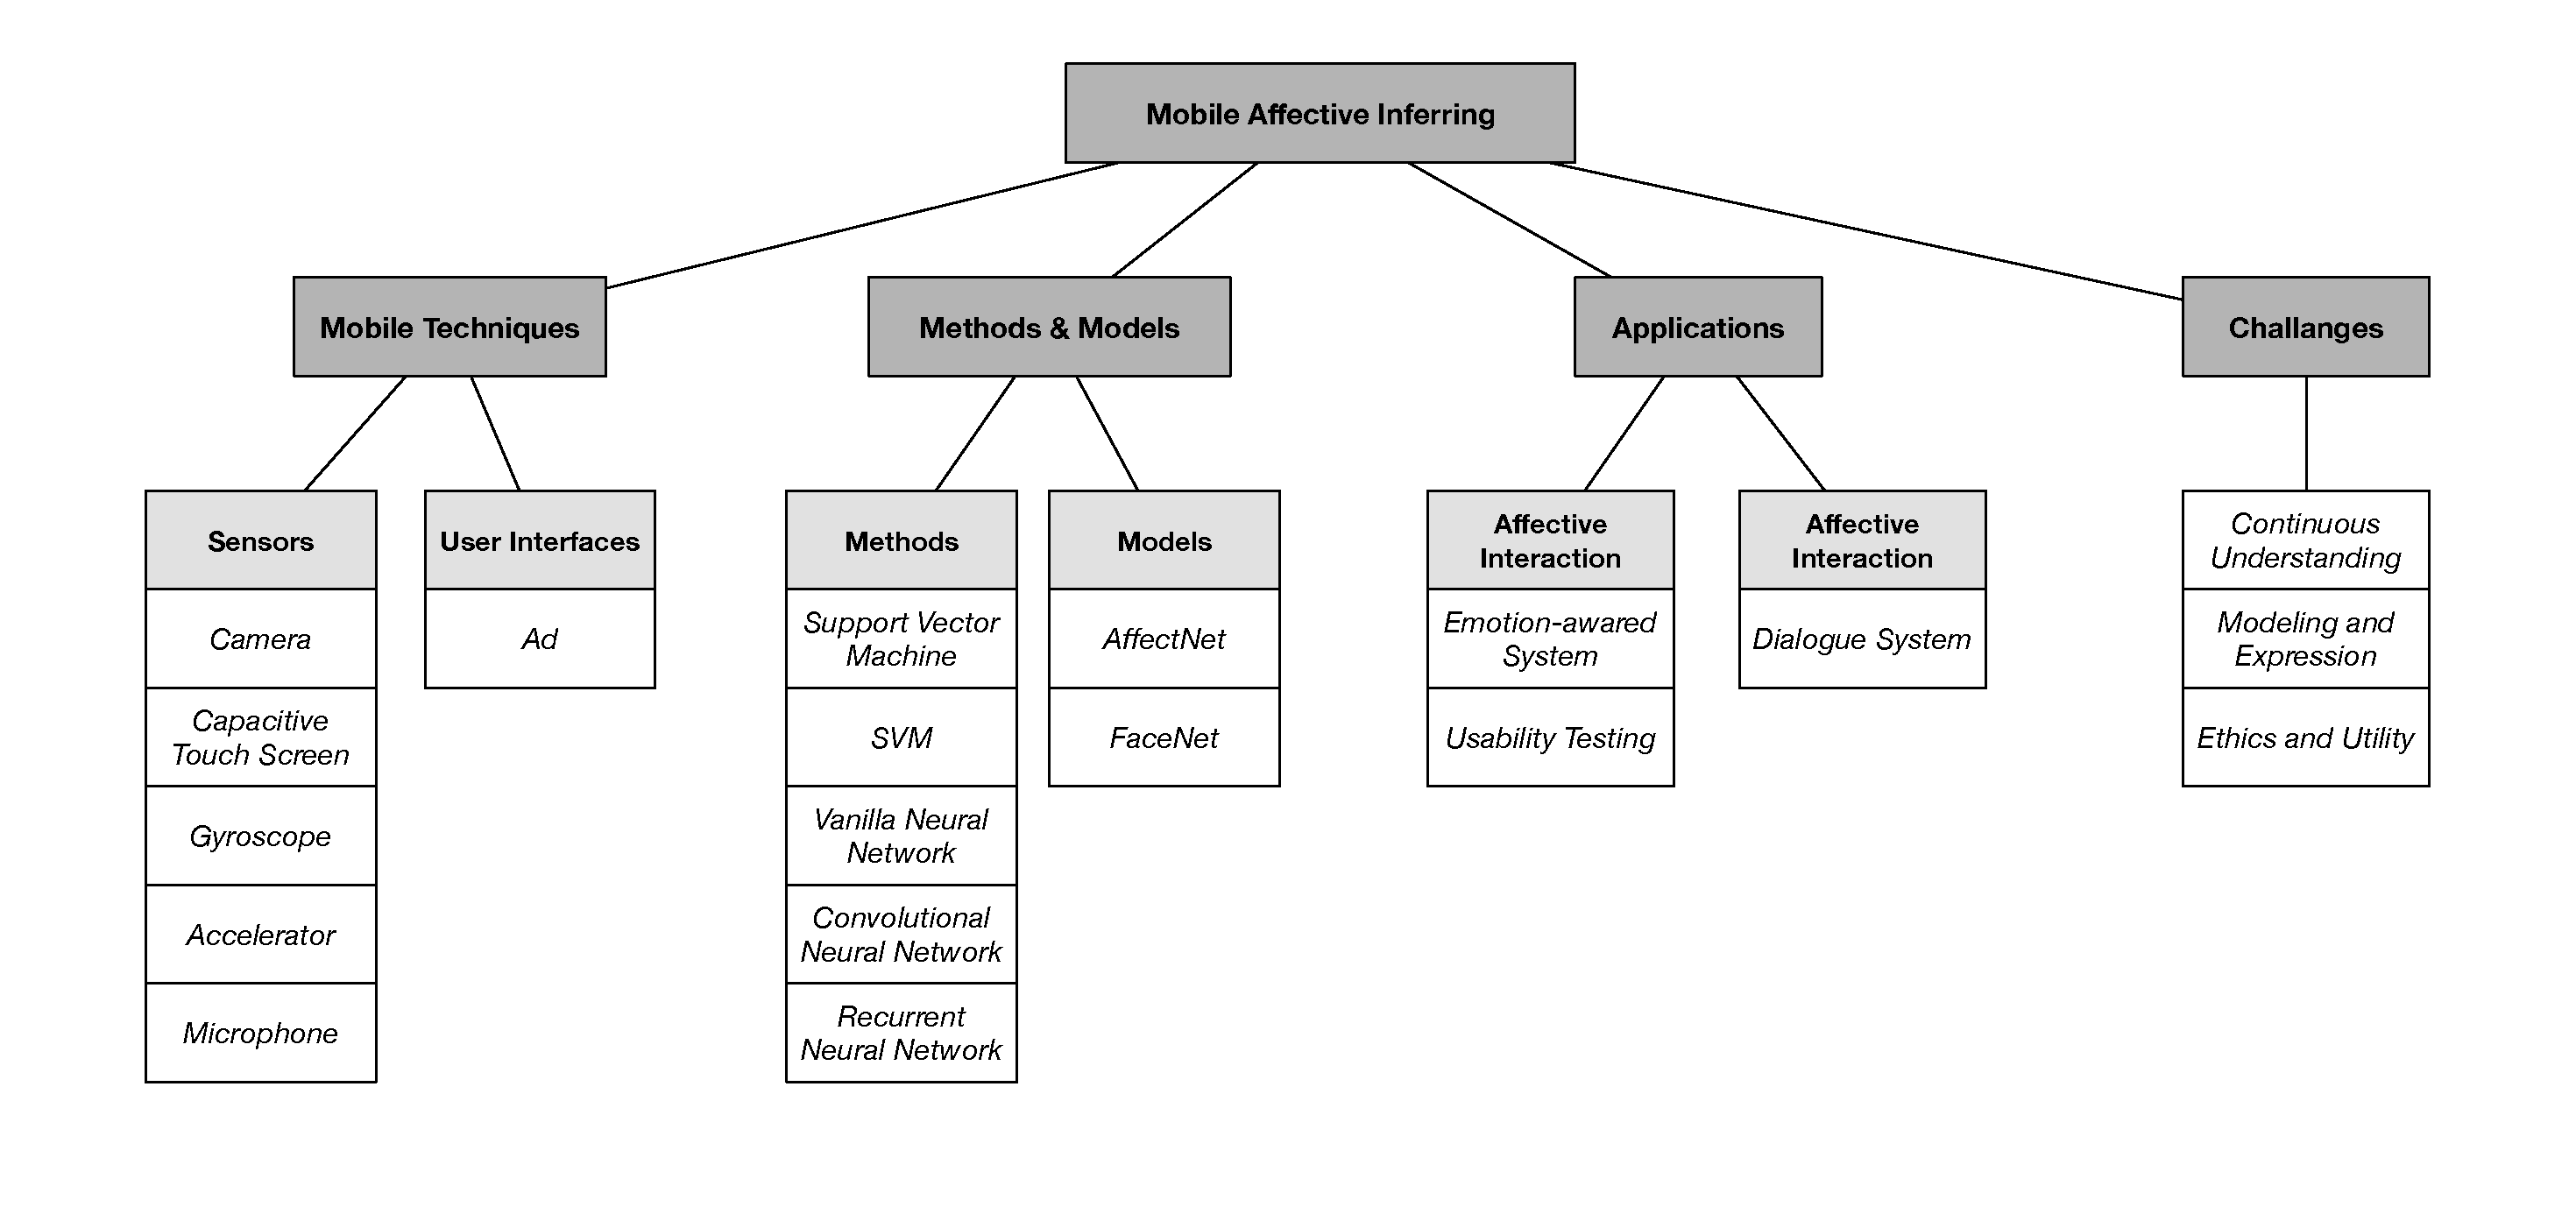
\includegraphics[width=0.5\textwidth]{hierarchical}
    \caption{Hierarchically-structured taxonomy of this paper.}
    \label{fig:hierarchically}
\end{figure}
\section{Data Sources}\label{sec:source}

- \cite{Tao2005} gives image for different information and different related sensing.
- \cite{Poria2017} gives multimodal considerations image. 90\% literature consider visual, audio and text information as multimodal affect analysis

\subsection{Camera}\label{subsec:vision}
We emphasis vision sensors in the first place since face and facial expressions are undoubtedly one of the most important nonverbal channels used by the human being to convey internal emotion. This part mainly discusses vision sensors, which includes RGB camera and depth camera, and illustrates how vision sensor can be used for affective emotion inferring.

Pure RGB cameras has been widely used in commercial smartphone as image sensor. 
For the camera with depth informations on mobile (recently introduced TrueDepth Camera in iPhone X \footnote{\url{https://www.apple.com/iphone-x/\#truedepth-camera}}) combines infrared camera, flood illuminator, proximity sensor, ambient light sensor, front facing camera and dot projector to provide depth images of facial information of a user.

\cite{}


\subsection{Touch Screen}\label{subsec:touch}
Capacitive touch screen provides touch position, touch pressure, touch angle through time within a specific application context
\cite{Hertenstein2009, Gao2012, Shah2015, bhattacharya2017predictive}
% 这一部分主要讨论如何使用触摸传感器,可以触摸传感器的不同类型,研究项目中都是怎样使用触摸传感器的特征的?
% 几个可能的方面
% 1. 有文章显示 touch 行为可以进行情感交流 \cite{Hertenstein2009}
% 2. 在特定的应用情境下,有文章显示 touxh 行为可以推导当前的用户情感..cite???  这篇文章则提出了
% 3. 有文章首先总结了 haptic-based affect detection remains an understudy topic; \cite{Bhattacharya2017}
% 4. 既然触摸行为在表达情感上具有重要的指示,那么反过来如何用通过触摸来表达情感\cite{Lentini2017}\cite{Mazzoni2016}
This part mainly discusses touch sensors, which includes capacitive touch screen and 3D touch screen.
And also explain why touch sensor can be used for affective computing (they are applicable
because of specific application context), mainly cite these papers: ...

\subsection{Motion Sensors}\label{subsec:motion}
Motion sensors typically combines gyroscope and accelerometer, with this combination they can also provide device attitude
This part illustrate \cite{Rana, Mottelson2016, Bailenson2007}


\begin{itemize}
    \item \cite{Mottelson2016}: studied the implications of
    human affect on general purpose touch-based mobile interaction and showed that it is possible to detect mobile users’ positive and neutral affective states.
\end{itemize}

Motion sensors become important because it could tells us what is user's body language.

\subsection{Microphone}\label{subsec:audio}
Audio sensor usually refers to built-in microphones, it collects voice information from current environments, which can infers user emotions based on their speech contents

Audio sensors mainly infers to input and output microphones. This leans two part of affective computing:

First is inferring emotions from user speech. 
This task can also split as two part of inferring task, and one is directly infer from voice;
another is recognize speech text from user, then understanding or inferring from text.

Second is output a emotional speech from machines.

\subsection{GPS}\label{subsec:gps}
GPS sensors provides geographical information of a user. With Location Based Services, user emotion can be inferred by their location

\subsection{Application Context}\label{subsec:ui}
\section{Methods}\label{sec:methods}

Emotion inferring problem are mostly consider as a classification problem, which classifies three state of user emotion: Happy, Unhappy, Neutral. The reason of this consideration is argued by in technical constrains: more type of emotion we need to classify with more data we need to prepare.  In this section, we will see the most accurate technical method, models and their datasets in different data type aspects essentially all based on machine learning methods.

\subsection{Vision Aspect} \label{subsec:vision-model}

% 介绍普通和深度两种识别
The normal RGB camera brings us focusing on how conduct emotion recognition with RGB images. Through depth camera was recently introduced on commercial mobile phone, its principle basically as same as Microsoft Kinect (see Figure \ref{fig:kinect}). Considering these two different sensor aspects, we dive into two different research area on vision sensors.

\begin{figure}
  \centering
  \includegraphics[width=0.5\textwidth]{kinect}
  \caption{Principle of Microsoft Kinect.}
  \label{fig:kinect}
\end{figure}

\subsubsection{Plain recognition}

% 先介绍 最近的 CNN 方法
Recently, convolutional neural networks (CNNs) has successfuly make break-through contributions to computer vision as well as its application to emotion inferring. 
AlexNet \cite{Krizhevsky2012} popularized deep convolutional neural networks by winning the ImageNet Challenge. Subsequently, other powerful CNN architecture was proposed such as VGG\cite{Simonyan2015}, Inception series\cite{Szegedy2014, Szegedy2015, Szegedy2016}, ResNet\cite{He2016}, DenseNet\cite{iandola2014densenet} and CapsNet\cite{sabour2017dynamic}. However, the most accurate CNNs usually have hundreds of
layers and thousands of channels whereas it is entirely not possible to deploy them to mobile system. The increasing of mobile emotion inferring needs of running high quality deep neural networks on embedded devices encourage the study on efficient model designs\cite{he2015convolutional}. 

% 再介绍移动设备上模型的优化是非常重要的
SqueezeNet \cite{iandola2016squeezenet} is the first model that reduces parameters and computation significantly while maintaining accuracy. MobileNet \cite{howard2017mobilenets} and ShuffleNet \cite{zhang2017shufflenet} utilizes the depthwise separable convolutions among lightweight models. Table \ref{tab:cnn} shows the complexity comparation of these CNNs.

% 比较模型之间的性能
\begin{table}[htb]
  \caption{Complexity comparison of CNN models, smaller number refers good performance}
  \label{tab:cnn}
  \scriptsize
  \begin{center}
    \begin{tabular}{cccc}
      Model & Cls. Error (\%) &  Complexity (MFLOPs) \\
    \hline
    AlexNet\cite{Krizhevsky2012}                   & 42.8         &  720    \\
    SqueezeNet\cite{iandola2016squeezenet}                & 42.5         &  833    \\
    MobileNet\cite{howard2017mobilenets}                 & 31.6         &  325    \\
    ShuffleNet\cite{zhang2017shufflenet}                & 31.0         &  292    \\
    VGG-16\cite{Simonyan2015}                    & 28.5         & 15300
    \end{tabular}
  \end{center}
\end{table}

% 在识别之前首先需要定位到面部,这就涉及到 landmark detection
The classification on RGB images is just the final step of feedforward propagation. To determine the facial information inside a image essentially become more difficualt then just a classification, then the problem refers to Landmark detection.
The recent break-through contributions in these area is the Region-based CNN (R-CNN) approach \cite{girshick2014rich} that to bounding-box object detection is to attend to a manageable number of candidate object regions and the state-of-the-art approach Mask-R-CNN \cite{he2017mask} serve a conceptually simple, flexible, and general framework for object instance segmentation.

% 最后给出最新的 AffectNet 作为 vision 训练的 database
With all these computer vision methods, the ICML 2013 Challenges in Representation Learning introduced the Facial Expression Recognition 2013 (FER-2013)
database \cite{goodfellow2013challenges}. Fortunately human actors/subjects databases portray the basic emotions of human external emotion has been created, which solves the problem of training data.

Benitez-Quiroz et al. \cite{fabian2016emotionet} proposed EmotioNet database that extract features by using Gabor filters, their database is subject-independent and cross-database experiments.
\cite{mollahosseini2016facial} uses FER-Wild database, and trained them on AlexNet with noise estimation methods and archived 82.12\% accuracy on FER-Wild. 
AffectNet \cite{Mollahosseini2017} is the state-of-the-art database that proposed for given the largest database of facial expression, valence, and arousal in the wild (see Figure \ref{fig:affectnet}). In their paper, various evaluation metrics shows that their deep neural network gives the state-of-the-art performance in facial emotion recognition.

\begin{figure}
  \centering
  \includegraphics[width=0.5\textwidth]{affectnet}
  \caption{Samples of AffectNet database and classification results. The emotion expression labels is written in parentheses.}
  \label{fig:affectnet}
\end{figure}

\subsubsection{Depth recognition}

As we discussed in previous section, depth camera principle basically as same as Microsoft Kinect, the main difference between depth camera and RGB camera is it provides 3D ficial informations, which leads the model difference in this field. Unlike Kinect, depth camera in most cases can only provides ficial recostruction model information instead of body gesture. Thus, depth recognition mainly focuses on modelling 3D ficial points. 

Paper \cite{chen20153d} was the recent paper that considering 3D modelling. They propose a real-time 3D model-based method that continuously recognizes dimensional emotions from facial expressions in natural communications. The most challenge parts of their research covers the 3D facial informations reconstructed from 2D images. Zhang et al. \cite{zhang2016emotion} proposed their exploration on 3D ficial points modelling of emotion recognition that directly get depth information from Kinect, however their recognition only gives three difference state recognition.

Despite there already exists despth camera in mobile phone, researches in this area are rare and not in popular demand. We belive that main reason is 3D modelling requires extensive computation which is not possible from mobile devices at the moment.

\subsection{Voice Aspect}\label{subsec:voice-model}

Voice Aspect as we discussed in the previous section, emotion inferring from user speech is basically processing user speech. The first part is to inferring user speech text from their voice, and the second part of recognition is calculate sentiment from these texts.

\subsubsection{Speech recognition}

Speech recognition is a board research area and there exists extensive approaches to archive this goal. Previous years commercial systems modelling speech recognition by using Hiden markov model which archived good performance, however with the raising of deep learning methods, recurrent neral network \cite{mikolov2010recurrent}, Long-shor term memory cell \cite{hochreiter1997long} and attention machanism \cite{google2017}. It is hard to say which is the state-of-the-art model since speech recognition is much more complex than a typical vision task. Consider there are very successful commercial system such as Google Speech API \footnote{\url{https://cloud.google.com/speech/}}can performs stream speech recognition with returning the speech text information. We don't consider this area in detail for the mail goal of mobile affective computing.

\subsubsection{Sentiment Analysis}

Sentiment analysis requires text understanding and it is not an easy problem to
solve. Some machine learning techniques, including various supervised and unsupervised algorithms, are being utilized. Some algorithms rank the importance of sentences within the text and then construct a summary out of important sentences, others are endto-end generative models. After we have the speech text from user, sentiment analysis can be performed to evaluate user emotions for each speech sentence or a chunk of speech contents during a time period.

\cite{Rajalakshmi2017ACS} provides a board and comprehensively survey on sentiment analysis. We conclude here for the general steps of sentiment analysis:

The approach to extract sentiment from speech text is
as follows:
\begin{itemize}
  \item Tokenize each word via a public sentiment calculation dataset;
  \item For each word, compare it with positive
  sentiments and negative sentiments word
  in the dictionary. Then increment positive
  count or negative count.
  \item Finally, based on the positive count and
  negative count, once can get result percentage about sentiment to decide the
  polarity.
\end{itemize}

Sentiment calculation for text essentially a clear defined engineering and the final re sentiment valuesults of user speech can be a training feature to different modalities.

\subsection{Touch Aspect}\label{subsec:touch-model}

Touch interaction modality in previous research all considered using handcrafted feature for touch behaviour and using kernel SVM to train linear models for classification. \cite{Gao2012} is the fisrt application specific in game, which the recognition rates are very robust even in naturalistic settings in the context of smartphone-based computer games. 
\cite{Shah2015} proposed a reasonable hand crafted features, for three classes (happy, unhappy, neutral); The recent studies in \cite{bhattacharya2017predictive} has 7 proposed features, for four classes (Excited, Relaxed, Frustrated, Bored) classification; and \cite{Tikadar2017} compares four discriminative models, namely the Naïve Bayes, K-Nearest Neighbor (KNN), Decision Tree and Support Vector Machine (SVM) were explored, with SVM giving the highest accuracy of 96.75\%. Table \ref{tab:touch-feature} shows a feature set of touch interaction information and Table \ref{tab:touch-cls} shows the performance comparation for different classifiers. However readers should incase that these provides solution doesn't provide any stability analysis of their classification model, it is possbile can be counter as a overfitting if readers cannot recur the accuracy.

\begin{table}
  \caption{Comparison of classifiers.}
  \label{tab:touch-feature}
  \scriptsize
  \begin{center}
    \begin{tabular}{lll}
      Feature & Unit (\%)\\
    \hline
    Deviation in number of strikes & \\
    Deviation in number of taps & \\
    Mode of strike length & Millimeter \\
    Average strike length & Millimeter \\ 
    Mode of strike speed  & Meter/second \\ 
    Average strike speed  & Meter/second
    Mode of delay & Millisecond \\
    Average delay & Millisecond \\ 
    Total delay   & Second\\
    Turnaround time & Second\\
    \end{tabular}
  \end{center}
\end{table}

\begin{table}
  \caption{Comparison of classifiers.}
  \label{tab:touch-cls}
  \scriptsize
  \begin{center}
    \begin{tabular}{lll}
      Classifier & Accuracy (\%) \\
    \hline
    Naïve Bayes     & 86.13\%           \\
    kNN                & 92.82\%       \\
    SVM                 & 96.75\%         \\
    \end{tabular}
  \end{center}
\end{table}

Touch interaction is a typical interaction information on mobile which output from users.
One can conclude here is SVM as the most accurate model for handcrafted model in this research direction.


\subsection{Sensors Fusion}\label{subsec:fusion}

Motimodal fusions of previous sensors is essentially a complex challenge. Many many research has foducs on this analysis, in particular \cite{Zeng2004} gives bimodal affective recognition via ficial emotion recognition and combined audio with visual modalities so that the final affect recognition accuracy is greatly improved to almost 90\%. \cite{Dermody2016} proposed a multimodal system with real-time feedback for publick speaking. The system has been developed within the paradigm of positive computing which focuses on designing for user wellbeing.

As multimodal sentiment analysis and emotion recognition research continues to gain popularity among the AI and NLP research communities, there is need for a timely, thorough literature review to define future directions, which can, in particular, further the progress of early stage researchers interested in this multidisciplinary field (see Figure \ref{fig:multimodal}).

\begin{figure}
  \centering
  \includegraphics[width=0.5\textwidth]{multimodal}
  \caption{A typical multimodal affect analysis framework, image from \cite{Poria2017}.}
  \label{fig:multimodal}
\end{figure}

The recent surveys of multimodal affect analysis on mobile \cite{d2015review, poria2016fusing, Poria2017},
focuses mainly on the state of the art in collecting sample data, and reports performance comparison of selected multimodal and unimodal systems, as opposed to comprehensively reviewing key individual systems and approaches, from the growing literature in the field.

Table \ref{tab:feature-level} from \cite{d2015review} shows the most commonly used experiments result of fusion modalities.


\begin{table}
  \tiny
  \caption{Results of feature-level fusion}
  \label{tab:feature-level}
  \scriptsize
  \begin{center}
    \begin{tabular}{lll}
      Combination of modalities & Precision  \\
    \hline
    Accuracy of the experiment carried out on Textual Modality & 0.619   \\
    Accuracy of the experiment carried out on Audio Modality   & 0.652  \\
    Accuracy of the experiment carried out on Vision Modality   & 0.681  \\
    Experiment using only visual and text-based features       & 0.7245 \\
    Result obtained using visual and audio-based features      & 0.7321 \\
    Result obtained using audio and text-based features        & 0.7115 \\
    Accuracy of feature-level fusion of three modalities       & 0.782 
    \end{tabular}
  \end{center}
\end{table}

On the same training and test sets, the classification
experiment using SVM, ANN and ELM. ELM outperformed ANN by
12\% in terms of accuracy (see Table \ref{tab:classifier}).
In terms of training time, the ELM outperformed SVM and ANN
by a huge margin (Table 7). A real-time multimodal sentiment analysis engine, 
the ANN as a classifier which provided the best performance in
terms of both accuracy.

\begin{table}
  \caption{Comparison of classifiers.}
  \label{tab:classifier}
  \scriptsize
  \begin{center}
    \begin{tabular}{lll}
      Classifier & Recall (\%) & Training time \\
    \hline
    SVM                   & 77.03         &  2.7 min    \\
    ELM                & 77.10         &   25 s    \\
    ANN                 & 57.81         &  2.9 min    \\
    \end{tabular}
  \end{center}
\end{table}

In conclusion, we discussed the technique method in different method. We conclude here in this section for each type of data:

\begin{itemize}
  \item \emph{Vision data}: CNN models performs the state-of-the-art performance of facial analysis;
  \item \emph{Speech data}: RNN models performs the state-of-the-art performance of speech recognition and sentiment analysis;
  \item \emph{Interaction data}: handcrafted features are the most commonly used feature and neural networks for these kind of unstructured data are unminded;
  \item  \emph{Context data}: application context and geographic location are normally use as a validation dimension for emotion inferring, researches doesn't consider them how to properly use as a training feature.
\end{itemize}
\section{Applications}
\label{sec:applications}
\subsection{Dialogue \& Chatbot system}
\subsubsection{Affective Interaction}
\cite{Conati2005, Hutchison2011}

\subsection{Emotion-awared system}
\subsubsection{Adaptive User Interfaces}
\cite{Dalvand, Galindo, Kaiser2006}
\subsubsection{Usability Testing}

\section{Challenges and Limitations}\label{sec:challenges}

The primary limitation of traditional AC research refers to as impermeable emotions.

\cite{Picard2003}

\subsection{State Understanding}

Continuous emotion state understanding is much more challenge since its not related to external emotion but also related to internal emotions, various emotions can be expressed as follows map \textit{(see figure~\ref{fig:emotions})}.

\begin{figure}[htb]
    \centering
    \includegraphics[width=3.5in]{emotion-map}
    \caption{A map of human emotions~\cite{emotionmap}.}
    \label{fig:emotions}
\end{figure}
\section{Conclusions}
\label{sec:conclusion}

In this paper, we investigated the recent advances in mobile affective computing related to human-computer interaction projects and inference techniques.

Section~\ref{sec:source} addresses different data sources in various mobile commodity sensors for emotion inference in previous studies. These include camera, touch screen, motion sensors, microphone, GPS, and application context. 

Next, in the Section~\ref{sec:methods}, 
we first carried out the review of emotion inference methods based on different type of data source, and compared the tested methods and inference models from previous researchers. In these comparisons, we first reviewed various models for user emotion inference, researchers usually transfers emotion inference problem into a classification problem. As a classification problem, most researchers consider user emotions can be inferred to three different states (Happy, Unhappy, Neutral). In each subsection, we highlighted the most useful methods for different type of emotion inference that concluded by the most recent research papers, such as CNN as the best way of vision type, RNN as the best way of auditory type, and handcrafted feature with SVM as the best way of interaction details. At the end of this section, we considered the combinations of these types of data. According to our investigation, the most commonly used data type are suggested to \emph{vision and audio} data in mobile affective computing; However, the combination of \emph{vision, audio, interaction details, and context for aspects fusion are unmined open topics}.

In Section~\ref{sec:applications}, we survey two novel applications in human-computer interaction related projects driven by emotion inference. Voice user interfaces consider user emotion as inputs and suggest to please users by adjusting system voice tone; Adaptive graphics user interfaces then considers emotion state as the context of UI theme.

Despite we researched the scientific approaches of mobile emotion inference in human-computer interaction related topics, there still apparent challenges in this area. Section~\ref{sec:challenges} pointed out the current problems of this research area. The main challenges of this area are \emph{impermeable emotions} and \emph{continuous understanding}. Moreover, the generalisability of mobile affective computing applications are subject to certain limitations. For instance, most of \emph{inference models are context specific} and multimodal inference then \emph{requires large computation resources}.

Nowadays, new technologies and methods provide us new opportunities of affect emotion inference in an unobtrusive mobile device. Since the complexity of the interpretation of human behavior at a very deep level is tremendous and requires a highly interdisciplinary collaboration, we believe the true break-throughs application in this field can be established by precisely modeling and new sensing technologies in the future.

\nocite{*}
\printbibliography
\end{document}
